%\bigskip
%\hrule
%\smallskip
%\hfill Edited by Takayoshi Shoudai on 2024-05-18 (2nd version), 2024-10-30 (3rd version).
\newtheorem{prop}{Proposition}
\newcommand{\pair}[2]{(#1,#2)}
%\newcommand{\pair}[2]{#1#2}
\newcommand{\TheConditionA}{$b \not\in \{a,d\}$ and $c \not\in \{a,d\}$}
%\newcommand{\TheConditionA}{$bc \not\in \{aa, ad, da, dd\}$}
\newcommand{\TheConditionB}{$b \not\in \{d\} \mbox{~and~}c \not\in \{a,d\}$}
%\newcommand{\TheConditionB}{$bc \not\in \{da, dd\}$}
\newcommand{\TheConditionC}{$b \not\in \{a, d\} \mbox{~and~} c \not\in \{a\}$}
%\newcommand{\theconditionC}{$bc \not\in \{aa, da\}$}


\begin{prop}\label{prop:repstring_origin}
  Let $w$ be a string of constant symbols in $\Sigma$ and $a,b$ constant symbols in $\Sigma$.
  If
  \begin{align}
  wa & = bw\label{eq:repstring_origin}
  \end{align}
  holds, then $a = b$ holds.
\end{prop}

\begin{proof}
If $|w|=0$ or $1$, it is trivial. We assume that for a string of constant symbols $u$ with $|u| < |w|$, if $ua = bu$ then $a = b$ holds. When $|w| \geq 2$, since $b$ is a prefix of $w$, there exists a string of constant symbols $u$ such that $w = bu$. From $bua = bbu$, we have $ua = bu$. Thus, from the assumption, we have $a = b$.  
\end{proof}

\begin{prop}\label{prop:repstring_base}
Let $w$ be a string of constant symbols in $\Sigma$ and $a,b,c,d$ constant symbols in $\Sigma$.
If
\begin{align}
wda & = bcw\label{eq:repstring_base}
\end{align}
holds, then $\pair{b}{c} = \pair{a}{d}$ or $\pair{b}{c} = \pair{d}{a}$ hold.
\end{prop}

\begin{proof}
  We will prove this proposition by an induction on $|w|$.
  For $i=1,\ldots,|w|$, we refer the $i$-th symbol of $w$ as $w[i - 1]$. 
  \begin{enumerate}
  \item[(i)] $|w| = 0$: Directly from Eq.~(\ref{eq:repstring_base}), $\pair{b}{c} = \pair{d}{a}$ holds.
  \item[(ii)] $|w| = 1$: From $w[0]da = bcw[0]$, we have $w[0] = b$, $d = c$, and $a = w[0]$. Thus, $\pair{b}{c} = \pair{a}{d}$ holds.
  \item[(iii)] $|w| = 2$: From $w[0]w[1]da = bcw[0]w[1]$, we have $w[0] = b$, $w[1] = c$, $d = w[0]$, $a = w[1]$. Thus, $\pair{b}{c} = \pair{d}{a}$ holds.
  \item[(iv)] $|w| = 3$: From $w[0]w[1]w[2]da = bcw[0]w[1]w[2]$, we have $w[0] = b$, $w[1] = c$, $w[2] = w[0]$, $d = w[1]$, $a = w[2]$. Thus, $\pair{b}{c} = \pair{a}{d}$ holds.
  \item[(v)] $|w| \ge 4$: We assume that for any string $u$ with $0\leq |u| < n$, if $uda = bcu$ holds, $\pair{b}{c} = \pair{a}{d}$ or $\pair{b}{c} = \pair{d}{a}$ hold. Since the string $w$ has a prefix $bc$ and a suffix $da$, there exists a string $u$ with $|u| = |w| - 4 < |w|$ such that $w = bcuda$ holds. Since $wda = bcw$, we have $bcudada = bcbcuda$, and then $uda = bcu$. Thus, from the assumption, we get $\pair{b}{c} = \pair{a}{d}$ or $\pair{b}{c} = \pair{d}{a}$.
  \end{enumerate}
From the above, we conclude that if $wda = bcw$ holds, then $\pair{b}{c} = \pair{a}{d}$ or $\pair{b}{c} = \pair{d}{a}$ hold.
\end{proof}

The conclusion from Proposition~\ref{prop:repstring_base} shows that $\pair{a}{d} = \pair{b}{c}$ or $\pair{a}{d} = \pair{c}{b}$. Therefore, if the equation $daw = wbd$ holds, we arrive at the same conclusion.

\begin{prop}\label{prop:repstring}
Let $w,w^{\prime}$ be strings of constant symbols in $\Sigma$ and $a,b,c,d$ constant symbols in $\Sigma$.
If
\begin{align}
  wdaw^{\prime} & = w^{\prime}bcw\label{eq:repstring}
\end{align}
holds, then $\pair{b}{c} = \pair{a}{d}$ or $\pair{b}{c} = \pair{d}{a}$ hold.\label{prop:repstring_eq}
\end{prop}

\begin{proof}
We will prove this proposition by an induction on $|w| + |w^{\prime}|$.
Without loss of generality, we assume that $|w| \geq |w^{\prime}|$, because if $|w| > |w^{\prime}|$ holds, we arrive at the same conclusion: $\pair{a}{d} = \pair{b}{c}$ or $\pair{a}{d} = \pair{c}{b}$.
\begin{enumerate}
  \item[(i)] $|w| \geq 0$ and $|w^{\prime}|=0$:
  Eq.~(\ref{eq:repstring}) becomes $wda = bcw$. From Proposition~\ref{prop:repstring_base}, $\pair{b}{c} = \pair{a}{d}$ or $\pair{b}{c} = \pair{d}{a}$ hold.
\end{enumerate}
We assume that for constant strings $u$ and $u^{\prime}$ with $|u| + |u^{\prime}| < |w| + |w^{\prime}|$, if $udau^{\prime} = u^{\prime}bcu$ holds, then $\pair{b}{c} = \pair{a}{d}$ or $\pair{b}{c} = \pair{d}{a}$ hold.
We partition the relations between $|w|$ and $|w^{\prime}|$ into the following four parts:
\begin{enumerate}
\item[(ii)] $0 < |w^{\prime}| \le |w| \le |w^{\prime}|+1$:
When either $|w|=|w^{\prime}|$ or $|w|=|w^{\prime}|+1$, Eq.~(\ref{eq:repstring}) is depicted as shown in Figs.~\ref{追加部分7} and \ref{追加部分8}, respectively.
It When $|w|=|w^{\prime}|$, $\pair{b}{c} = \pair{d}{a}$ holds. When $|w|=|w^{\prime}|+1$, $a = c$ and $w = w^{\prime}b = dw^{\prime}$ hold.
From Proposition~\ref{prop:repstring_origin}, we get $b = d$.
Therefore, $\pair{b}{c} = \pair{a}{d}$ or $\pair{b}{c} = \pair{d}{a}$ hold.
%
\item[(iii)] $|w^{\prime}|+2 \le |w| \le 2|w^{\prime}| - 1$:
On Eq.~\ref{eq:repstring}, since $|wdaw^{\prime}| = |w^{\prime}bcw| = |w| + |w^{\prime}| + 2$, a suffix of $w$ overlaps with a prefix of $w$ as shown in Fig.~\ref{w1+3}.
That is, there exists a constant string $u$ of length $2|w| - (|w| + |w^{\prime}| + 2) = |w| - |w^{\prime}| - 2$ such that $u$ is a prefix and a suffix of $w$.
Since $uda$ is of length $|w| - |w^{\prime}|$, $uda$ is also a prefix of $w$. Similarly, $bcu$ is also a suffix of $w$.
Since $|w| - (|uda| + |bcu|) = 2|w| - |w^{\prime}| \ge 1$, there exist a constant string $u^{\prime}$ of length $2|w^{\prime}| - |w|$ such that $w = udavbcu$ holds.
Since $w^{\prime}$ is a suffix of $w$ and $|u^{\prime}bcu| = (2|w^{\prime}| - |w|) + 2 + (|w| - |w^{\prime}| - 2) = |w^{\prime}|$, we have $w^{\prime} = u^{\prime}bcu$.
Similarly, we have $w^{\prime} = udau^{\prime}$. Thus, we have a new equation $u^{\prime}bcu = udau^{\prime}$.
Since $|u| = |w| - |w^{\prime}| - 2 \leq |w| - 3 < |w|$ and $|u^{\prime}| = 2|w^{\prime}| - |w| < |w|$, i.e., $|u| + |u^{\prime}| < |w| + |w^{\prime}|$ holds, from the induction hypothesis on $|u| + |u^{\prime}|$, $\pair{b}{c} = \pair{a}{d}$ or $\pair{b}{c} = \pair{d}{a}$ hold.
%
\item[(iv)] $2|w^{\prime}| \le |w| \le 2|w^{\prime}|+3$:
When $|w|=2|w^{\prime}|$, we easily see that $w = w^{\prime}w^{\prime}$.
Therefore, $w^{\prime}da = bcw^{\prime}$ holds as shown in Fig.~\ref{追加部分14}. From Proposition~\ref{prop:repstring_base}, $\pair{b}{c} = \pair{a}{d}$ or $\pair{b}{c} = \pair{d}{a}$ hold.
When $|w|=2|w^{\prime}|+i$ ($i=1,2,3$), Eq.~(\ref{eq:repstring}) is depicted as shown in Figs.~\ref{追加部分13}, \ref{追加部分12}, and \ref{追加部分11}.
When $|w|=2|w^{\prime}|+2$, trivially we have $\pair{b}{c} = \pair{d}{a}$. 
When $|w|=2|w^{\prime}|+1$ and $|w|=2|w^{\prime}|+3$, from Proposition~\ref{prop:repstring_origin}, $\pair{b}{c} = \pair{a}{d}$ holds.
%
\item[(v)] $2|w^{\prime}|+4 \leq |w|$:
Since the strings $w^{\prime}bc$ and $adw^{\prime}$ are a prefix and a suffix of $w$, respectively, and $|w^{\prime}bc| + |adw^{\prime}| = 2|w^{\prime}| + 4$, there exists a string $u$ with $|u| \geq 0$ such that $w = w^{\prime}bcudaw^{\prime}$ holds.
From Eq.~(\ref{eq:repstring}), $w^{\prime}bcudaw^{\prime}daw^{\prime} = w^{\prime}bcw^{\prime}bcudaw^{\prime}$, i.e., $udaw^{\prime} = w^{\prime}bcu$ holds as shown in Fig.~\ref{2w1+5}.
Let $u^{\prime} = w^{\prime}$.
Since $|u| + |u^{\prime}| = |w|- (2|w^{\prime}| + 4) + |w^{\prime}| < |w| + |w^{\prime}|$, from the induction hypothesis on $|u| + |u^{\prime}|$, $\pair{b}{c} = \pair{a}{d}$ or $\pair{b}{c} = \pair{d}{a}$ hold.
\end{enumerate}
From the above, we conclude that if $wdaw^{\prime} = w^{\prime}bcw$, then $\pair{b}{c} = \pair{a}{d}$ or $\pair{b}{c} = \pair{d}{a}$ hold.
\end{proof}

\begin{figure}[t]
\begin{center}
  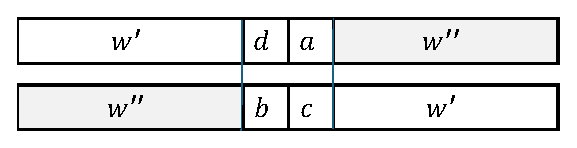
\includegraphics[scale=0.45]{figs/w=w_1.eps}
  \caption{Subcase $|w^{\prime}| = |w^{\prime\prime}|$ of (ii) of \textit{Claim} 5 (Lemma~\ref{追加部分})}\label{追加部分7}
  \bigskip
  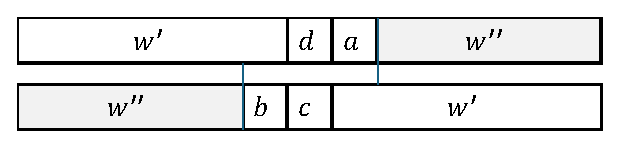
\includegraphics[scale=0.45]{figs/w=w_1+1.eps}
  \caption{Subcase $|w^{\prime}| = |w^{\prime\prime}| + 1$ of (ii) of \textit{Claim} 5 (Lemma~\ref{追加部分})}\label{追加部分8}
  %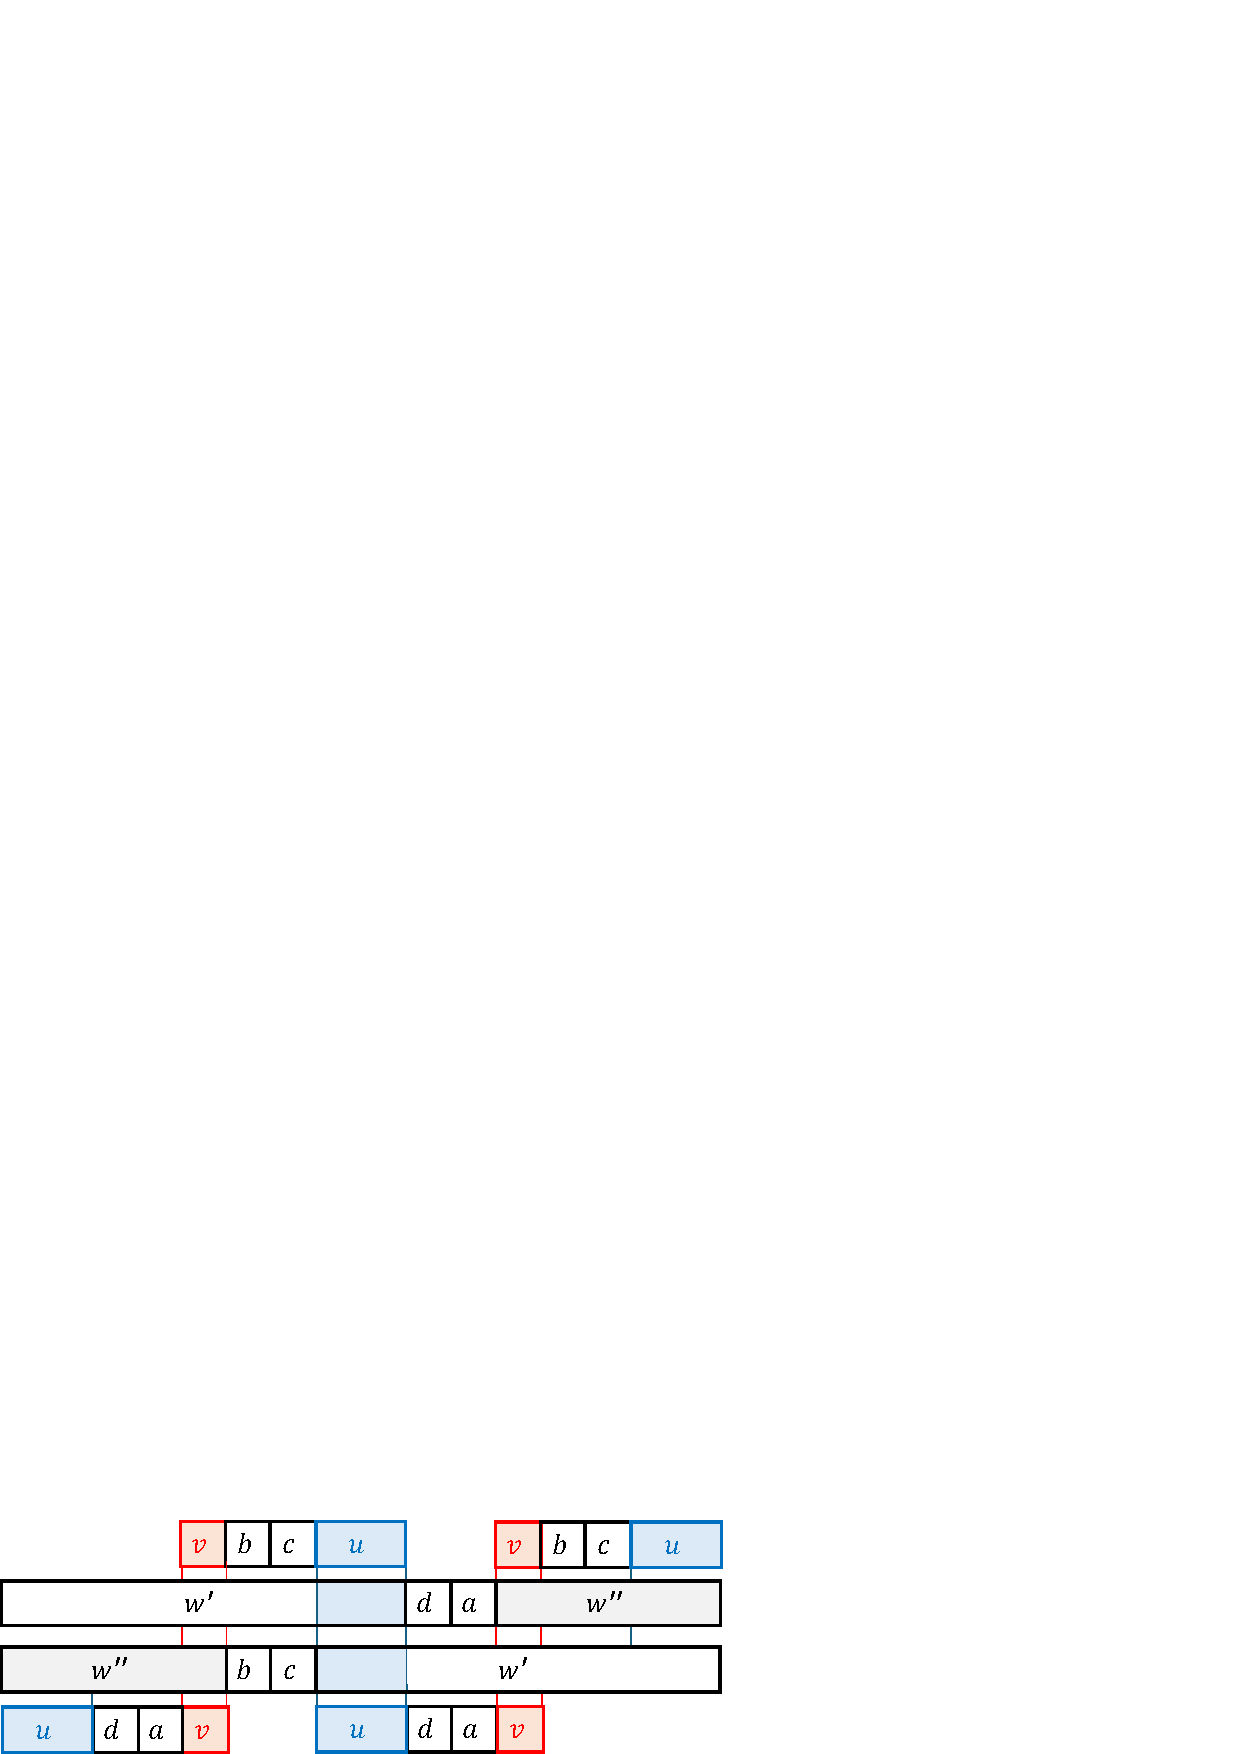
\includegraphics[scale=0.35]{figs/w=w_1+2.png}
  %\caption{Subcase $|w^{\prime}| = |w^{\prime\prime}| + 2$ of (ii) of \textit{Claim} 5 (Lemma~\ref{追加部分})}\label{追加部分9}
\end{center}
\end{figure}

\begin{figure}[t]
\begin{center}
  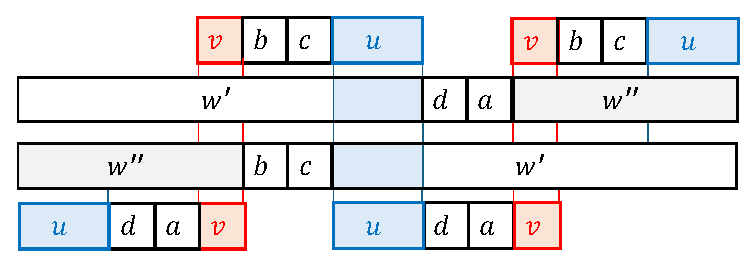
\includegraphics[scale=0.45]{figs/w=w_1+2.eps}
  \caption{Case $|w^{\prime\prime}| + 2 \le |w^{\prime}| \le 2|w^{\prime\prime}| - 1$ of (iii) of \textit{Claim} 5 (Lemma~\ref{追加部分})}\label{w1+3}
\end{center}
\end{figure}

\begin{figure}[t]
\begin{center}
  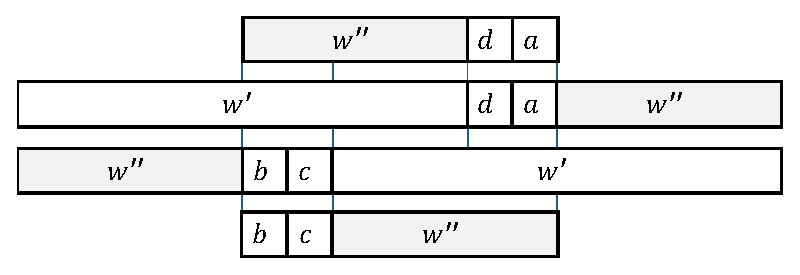
\includegraphics[scale=0.45]{figs/w=2w_1.eps}
  \caption{Subcase $|w^{\prime}| = 2|w^{\prime\prime}|$ of (iv) of \textit{Claim} 5 (Lemma~\ref{追加部分})}\label{追加部分14}
  \bigskip
  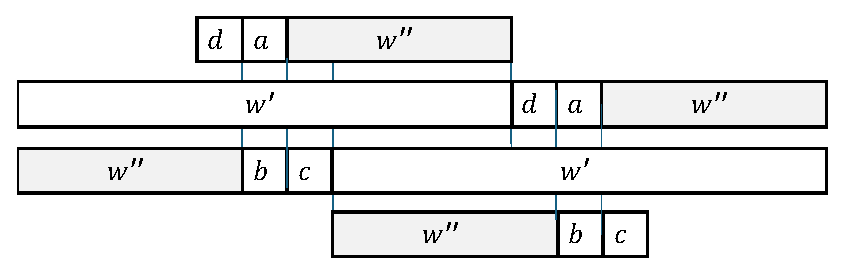
\includegraphics[scale=0.45]{figs/w=2w_1+1.eps}
  \caption{Subcase $|w^{\prime}| = 2|w^{\prime\prime}| + 1$ of (iv) of \textit{Claim} 5 (Lemma~\ref{追加部分})}\label{追加部分13}
  \bigskip
  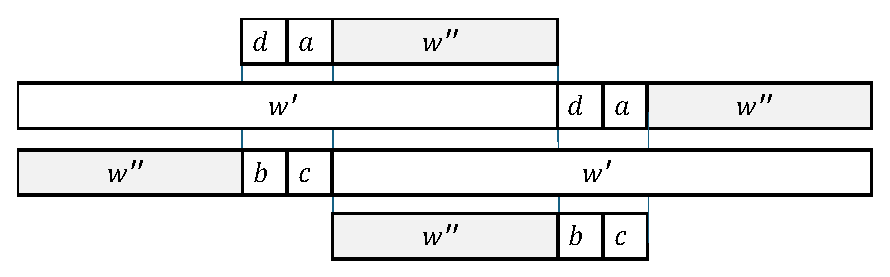
\includegraphics[scale=0.45]{figs/w=2w_1+2.eps}
  \caption{Subcase $|w^{\prime}| = 2|w^{\prime\prime}| + 2$ of (iv) of \textit{Claim} 5 (Lemma~\ref{追加部分})}\label{追加部分12}
  \bigskip
  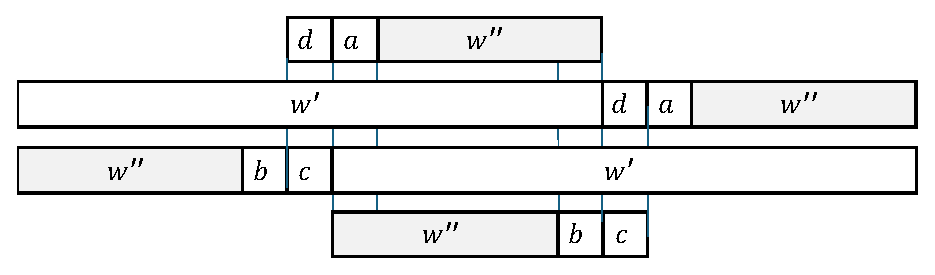
\includegraphics[scale=0.45]{figs/w=2w_1+3.eps}
  \caption{Subcase $|w^{\prime}| = 2|w^{\prime\prime}| + 3$ of (iv) of \textit{Claim} 5 (Lemma~\ref{追加部分})}\label{追加部分11}
  %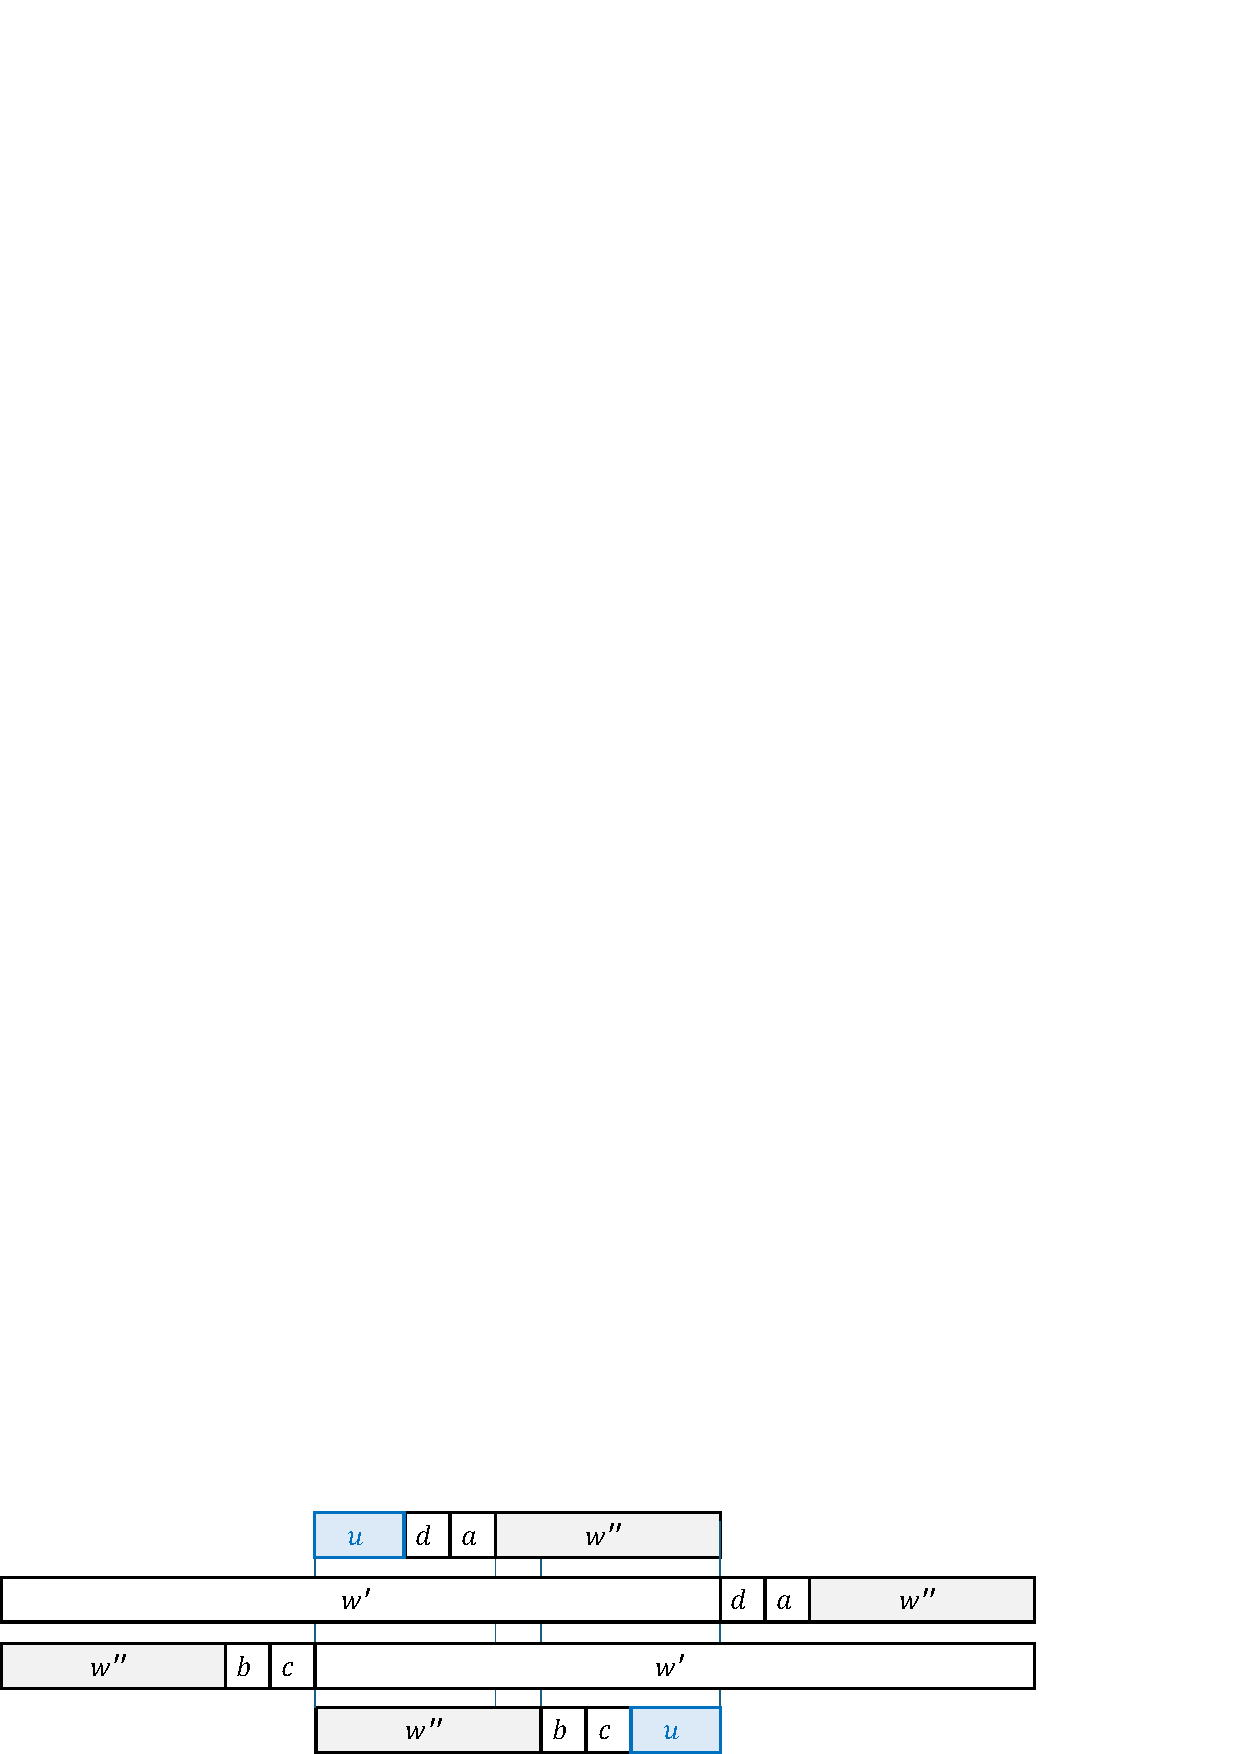
\includegraphics[scale=0.35]{figs/w=2w_1+4.png}
  %\caption{$|w| = 2|w_{1}|+4$における定数記号列}\label{追加部分10}
\end{center}
\end{figure}

\begin{figure}[t]
\begin{center}
  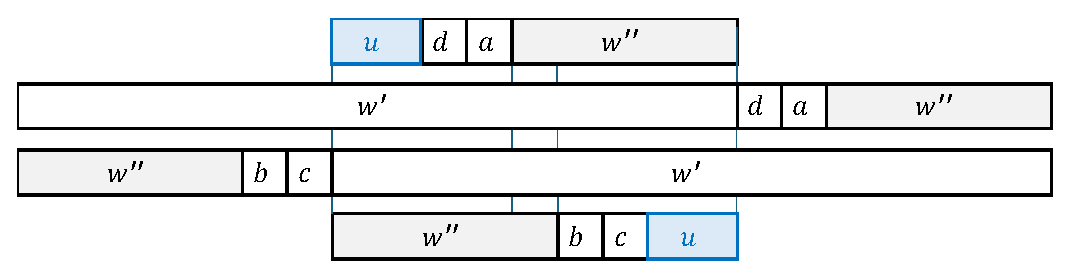
\includegraphics[scale=0.45]{figs/w=2w_1+4.eps}
  \caption{Case $2|w^{\prime\prime}| + 4 \leq |w^{\prime}|$ of (v) of \textit{Claim} 5 (Lemma~\ref{追加部分})}\label{2w1+5}
\end{center}
\end{figure}

\begin{lem}\label{追加部分}
  Let $\Sigma$ be an alphabet with $\sharp\Sigma \ge 3$ and $p,~q$ regular patterns on $\Sigma\cup X$.
  Let $D$ be the following set of regular patterns on $\Sigma\cup X$.
  Then, if $p \{ x := r \} \preceq q$ for all $r \in D$, then $p \{ x := xy \} \preceq q$:
  \begin{enumerate}
  \item[] $D = \{ ya, bc, dy \}$ (\TheConditionA).
  \end{enumerate}
\end{lem}

  \begin{proof}
  It is obvious if no variable symbol appears in $p$.
  Thus, for a variable symbol $x\in X$, let $p=p_{1}xp_{2}$, where each $p_{i}$ ($i=1,2$) is a regular pattern on $\Sigma\cup X$ or an empty symbol.
  We assume that $p \{ x := xy \} \not \preceq q$ in order to derive the contradiction.

  Since $p \{ x := r \} \preceq q$ for all $r \in D$, there are three strings of length $2$ corresponding to $ya, bc, dy$ in $q$.
  Note that the three strings may appear partly overlapping.
  The symbols appearing in $D$ corresponds to a variable or a constant symbol in $q$.
  Let $y_{1}, y_{2}, y_{3}$ be variable symbols appearing in $q$.
  The strings $ya$ and $dy$ must correspond to the strings $y_{1}a$ and $dy_{2}$ in $q$, respectively.
  There are the following three possibilities of strings in $q$ that corresponds to $bc$ in $p\{x:=bc\}$.
  \begin{center}
    \begin{tabular}{cccccc}
      \textrm{(a)} & $bc$, & \textrm{(b)} & $y_{3}c$, & \textrm{(c)} & $by_{3}$.
    \end{tabular}
  \end{center}

  Suppose that there exists (b) $y_{3}c$ in $q$ that corresponds to $bc$ in $p\{x:=bc\}$, i.e., there exist regular patterns $q_{1}$ and $q_{2}$ such that (1) $p_{1}bcp_{2} \preceq q_{1}y_{3}cq_{2}$, (2) either $p_{1} \preceq q_{1}$ or $p_{1} \preceq q_{3}y_{3}^{\prime}$ for some variable symbol $y_{3}^{\prime}\in X$, and (3) $p_{2} \preceq q_{2}$.
  In this case, it is easy to see that $p\{x:=yc\} = p_{1}ycp_{2} \preceq q_{1}y_{3}cq_{2}$ also holds. Thus, both $p\{x:=ya\}\preceq q$ and $p\{x:=yc\}\preceq q$ hold. Since $c\not= a$, from (ii) of Lemma \ref{two_variables}, $p\{x:=xy\}\preceq q$ holds. This contradicts the assumption. Similarly, the case (c) derives a contradiction from (i) of Lemma \ref{two_variables}.
  Therefore, in the following, we consider only the case of (a).

  Since $p \{ x := xy \} \not \preceq q$ and the condition \TheConditionA, the regular pattern $q$ can be expressed in one of the following forms: Let $y_{1}, y_{2}$ be distinct variable symbols in $X$ and $q_{1}, q_{2}, w, w^{\prime}$ either an empty string or a regular pattern on $\Sigma\cup X$.
  \begin{enumerate}
  \item[(a1)] $q=q_{1}AwBw^{\prime}Cq_{2}$, where $\{ A,B,C \} = \{ y_{1}a,bc,dy_{2} \}$.
  \item[(a2)] $q=q_{1}AwBq_{2}$, where $\{ A,B \} = \{ dy_{1}a,bc \}$.
  \item[(a3)] $q=q_{1}AwBq_{2}$, where $\{ A,B \} = \{ y_{1}ay_{2},bc \}$ ($a = d$).
  \end{enumerate}
  
  Firstly, we will consider the case (a1).

  \smallskip

  \noindent
  \textit{Claim} 1. $B \not\in \{y_{1}a, dy_{2}\}$.

  \smallskip
  \noindent
  \textit{Proof of Claim} 1.
  Suppose that $(A, B, C) = (dy_{2}, y_{1}a, bc)$. For some $y_{1}^{\prime},y_{2}^{\prime}\in X$, the following conditions hold:
  \begin{align*}
    \textrm{(1)}~& p_{1} \preceq q_{1} & \textrm{(1')}~& p_{2} \preceq wy_{1}aw^{\prime}bcq_{2}\mbox{ or} \\
    & & & p_{2} \preceq y_{2}^{\prime}wy_{1}aw^{\prime}bcq_{2}\\
    \textrm{(2)}~& p_{1} \preceq q_{1}dy_{2}w\mbox{ or}  & \textrm{(2')}~& p_{2} \preceq w^{\prime}bcq_{2}\\
    & p_{1} \preceq q_{1}dy_{2}wy_{1}^{\prime} & & \\
    \textrm{(3)}~& p_{1} \preceq q_{1}dy_{2}wy_{1}aw^{\prime} & \textrm{(3')}~& p_{2} \preceq q_{2}
  \end{align*}
  When $p_{2} \preceq wy_{1}aw^{\prime}bcq_{2}$ of (1') holds, let $q^{\prime}_{1}=q_{1}dy_{2},~q^{\prime}_{2}=wy_{1}aw^{\prime},~q^{\prime}_{3}=bcq_{2}$. Since $p_{1} \preceq q_{1}dy_{2}wy_{1}aw^{\prime}$ holds from (3), $p_{1} \preceq q^{\prime}_{1}q^{\prime}_{2}$ and $p_{2} \preceq q^{\prime}_{2}q^{\prime}_{3}$ hold and $q_{2}^{\prime}$ contains a variable symbol.
  %
  When $p_{2} \preceq y_{2}^{\prime}wy_{1}aw^{\prime}bcq_{2}$ of (1') holds, let $q^{\prime}_{1}=q_{1}d,~q^{\prime}_{2}=y_{2}wy_{1}aw^{\prime},~q^{\prime}_{3}=bcq_{2}$. Since $p_{1} \preceq q_{1}dy_{2}wy_{1}aw^{\prime}$ holds from (3), $p_{1} \preceq q^{\prime}_{1}q^{\prime}_{2}$ and $p_{2} \preceq q^{\prime}_{2}q^{\prime}_{3}$ hold and $q_{2}^{\prime}$ contains a variable symbol.
  In both cases, from Theorem~\ref{Sato1:Lemma9}, $p \preceq q$ holds. It contradicts the assumption that $p \{ x := xy \} \not \preceq q$.

  Similarly, we can show that any case of $(A, B, C) = (y_{1}a, dy_{2}, bc)$, $(bc, y_{1}a, dy_{2})$, $(bc, dy_{2}, y_{1}a)$ contradicts the assumption.
  %
  Therefore, we have $B \not\in \{y_{1}a, dy_{2}\}$. (\textit{End of Proof of Claim})

  \smallskip

  \noindent
  \textit{Claim} 2. $(A, B, C) = (y_{1}a, bc, dy_{2})$.

  \smallskip
  \noindent
  \textit{Proof of Claim} 2.
  From \textit{Claim} 1, we have $B=bc$. Suppose that $(A, B, C) = (dy_{2}, bc, y_{1}a)$, i.e., $q = q_{1}dy_{2}wbcw^{\prime}y_{1}aq_{2} $ holds. Then, the following conditions hold: for $y_{1}^{\prime},y_{2}^{\prime}\in X$,
  \begin{align*}
  \textrm{(1)}~& p_{1} \preceq q_{1} & \textrm{(1')}~& p_{2} \preceq wbcw^{\prime}y_{1}aq_{2}\mbox{ or}\\
  & & & p_{2} \preceq y_{2}^{\prime}wbcw^{\prime}y_{1}aq_{2}\\
  \textrm{(2)}~& p_{1} \preceq q_{1}dy_{2}w & \textrm{(2')}~& p_{2} \preceq w^{\prime}y_{1}aq_{2} \\
  \textrm{(3)}~& p_{1} \preceq q_{1}dy_{2}wbcw^{\prime}\mbox{ or} & \textrm{(3')}~& p_{2} \preceq q_{2}\\
  & p_{1} \preceq q_{1}dy_{2}wbcw^{\prime}y_{1}^{\prime}& &
  \end{align*}
 %
  From $p_{1} \preceq q_{1}dy_{2}w$ of (2), for some $p^{\prime}_{1}$ and $p^{\prime\prime}_{1}$, $p_{1}$ is expressed as $p^{\prime}_{1}p^{\prime\prime}_{1}$, where $p^{\prime}_{1} \preceq q_{1}d$ and $p^{\prime\prime}_{1} \preceq y_{2}w$. 
  When $p_{2} \preceq wbcw^{\prime}y_{1}aq_{2}$ of (1'), we have $p=p_{1}xp_{2}=p^{\prime}_{1}p^{\prime\prime}_{1}xp_{2} \preceq q_{1}dp^{\prime\prime}_{1}xwbcw^{\prime}y_{1}aq_{2}=q \{ y_{2}:=p^{\prime\prime}_{1}x \}$. Thus, $p \{ x := xy \} \preceq q \{ y_{2}:=p^{\prime\prime}_{1}xy \}$ holds. It contradicts the assumption that $p \{ x := xy \} \not \preceq q$.
  %
  When $p_{2} \preceq y_{2}^{\prime}wbcw^{\prime}y_{1}aq_{2}$ of (1'), we have $p=p_{1}xp_{2}=p^{\prime}_{1}p^{\prime\prime}_{1}xp_{2} \preceq q_{1}dp^{\prime\prime}_{1}xy_{2}^{\prime}wbcw^{\prime}y_{1}aq_{2}=q \{ y_{2}:=p^{\prime\prime}_{1}xy_{2}^{\prime} \}$.
  Thus, $p \{ x := xy \} \preceq q \{ y_{2}:=p^{\prime\prime}_{1}xyy_{2}^{\prime} \}$ holds. It also contradicts the assumption.
  %
  Therefore, we have $(A, B, C) = (y_{1}a, bc, dy_{2})$.
  (\textit{End of Proof of Claim})

  \smallskip

  From \textit{Claim} 2, $q$ is expressed as $q_{1}y_{1}awbcw^{\prime}dy_{2}q_{2}$, where \TheConditionA.
  If $p \{ x := xy \} \not \preceq q$ holds, we have the following conditions:
  for $y_{1}^{\prime},y_{2}^{\prime}\in X$,
  \begin{align*}
    \textrm{(1)}~& p_{1} \preceq q_{1} \mbox{ or} p_{1} \preceq q_{1}y_{1}^{\prime} & \textrm{(1')}~& p_{2} \preceq wbcw^{\prime}dy_{2}q_{2} \\
    \textrm{(2)}~& p_{1} \preceq q_{1}y_{1}aw & \textrm{(2')}~& p_{2} \preceq w^{\prime}dy_{2}q_{2} \\
    \textrm{(3)}~& p_{1} \preceq q_{1}y_{1}awbcw^{\prime} & \textrm{(3')}~& p_{2} \preceq q_{2} \mbox{ or} p_{2} \preceq y_{2}^{\prime}q_{2}
  \end{align*}

  \smallskip

  \noindent
  \textit{Claim} 3. $w$ and $w'$ contains no variable symbol.

  \smallskip
  \noindent
  \textit{Proof of Claim} 3.
  Let $q_{1}^{\prime} = q_{1}y_{1}a$, $q_{2}^{\prime} = wbcw^{\prime}$, and $q_{3}^{\prime} = dy_{2}q_{2}$. From (1') and (3), $p_{1} \preceq q^{\prime}_{1}q^{\prime}_{2}$ and $p_{2} \preceq q^{\prime}_{2}q^{\prime}_{3}$. If $q_{2}^{\prime}$ contains a variable symbol, from Theorem~\ref{Sato1:Lemma9}, $p \preceq q$ holds. It contradicts the assumption. Therefore, $w$ and $w'$ contains no variable symbol. (\textit{End of Proof of Claim})

  \smallskip

  From \textit{Claim} 3, $w$ and $w'$ are strings consisting of symbols in $\Sigma$. From (1') and (2'), $wbcw^{\prime}d$ and $w^{\prime}d$ are prefixes of $p_{2}$, and from (2) and (3), $awbcw^{\prime}$ and $aw$ are suffixes of $p_{1}$.
  From these facts, if $|w|=|w^{\prime}|$, $b = d$ and $a = c$ hold, and if $|w|=|w^{\prime}|+1$, $a = b$ holds.
  If $|w| = |w^{\prime}|+2$, since $awbcw^{\prime}$ and $aw$ are suffixes of $p_{1}$, and since $|w|\geq 2$, $a$ is a suffix of $w$.
  From (1') and (2'), since $wbcw^{\prime}d$ and $w^{\prime}d$ are prefixes of $p_{2}$, we have $w=w^{\prime}da$.
  Since $awbcw^{\prime}$ and $aw$ are suffixes of $p_{1}$, we have $w=bcw^{\prime}$.
  Thus, $w^{\prime}da = bcw^{\prime}$ holds.
  From Proposition~\ref{prop:repstring_base}, $\pair{b}{c} = \pair{a}{d}$ or $\pair{b}{c} = \pair{d}{a}$ hold.
  Therefore, these cases contradict the conditions \TheConditionA.
  From (2) and (3), if $|w| \ge |w^{\prime}|+3$, there exists a string $w^{\prime\prime}$ of length $|w|-|w^{\prime}|-2$ such that $w=w^{\prime\prime}bcw^{\prime}$ holds.
  Moreover, from (2) and (3), since $|aw| < |wbcw^{\prime}|$ and $aw = aw^{\prime\prime}bcw^{\prime}$, $aw^{\prime\prime}$ is a suffix of $w$.
  On the other hand, from (1') and (2'), $w^{\prime}d$ is a prefix of $w$.
  Since $|w^{\prime}d| + |aw^{\prime\prime}| = |w^{\prime}| + |w^{\prime\prime}| + 2 = |w|$, we have $w=w^{\prime}daw^{\prime\prime}$. Therefore, $w^{\prime}daw^{\prime\prime} = w^{\prime\prime}bcw^{\prime}$ holds.
  From Proposition~\ref{prop:repstring}, we have $\pair{b}{c} = \pair{a}{d}$ or $\pair{b}{c} = \pair{d}{a}$.
  It contradicts the conditions \TheConditionA.

  From the above, we conclude that all cases of (a1) contradict the assertion that $p\{x := xy\} \not\preceq q$ and that \TheConditionA.
  
  Secondly, for the case (a2), we suppose that $(A, B) = (dy_{1}a, bc)$, i.e., $q = q_{1}dy_{1}awbcq_{2} $ holds. Then, the following conditions hold: for $y_{1}^{\prime}\in X$,
  \begin{align*}
    \textrm{(1)}~& p_{1} \preceq q_{1} & \textrm{(1')}~& p_{2} \preceq awbcq_{2}\mbox{ or} \\
    & & & p_{2} \preceq y_{1}^{\prime}awbcq_{2}\\
    \textrm{(2)}~& p_{1} \preceq q_{1}d\mbox{ or}  & \textrm{(2')}~& p_{2} \preceq wbcq_{2}\\
    & p_{1} \preceq q_{1}dy_{1}^{\prime} & & \\
    \textrm{(3)}~& p_{1} \preceq q_{1}dy_{1}aw & \textrm{(3')}~& p_{2} \preceq q_{2}
  \end{align*}
  %
  From $p_{1} \preceq q_{1}dy_{1}aw$ of (3), for some $p^{\prime}_{1}$ and $p^{\prime\prime}_{1}$, $p_{1}$ is expressed as $p^{\prime}_{1}p^{\prime\prime}_{1}$, where $p^{\prime}_{1} \preceq q_{1}d$ and $p^{\prime\prime}_{1} \preceq y_{1}aw$. 
  When $p_{2} \preceq awbcq_{2}$ of (1'), we have $p=p_{1}xp_{2}=p^{\prime}_{1}p^{\prime\prime}_{1}xp_{2} \preceq q_{1}dp^{\prime\prime}_{1}xawbcq_{2}=q \{ y_{1}:=p^{\prime\prime}_{1}x \}$.
  Thus, $p \{ x := xy \} \preceq q \{ y_{1}:=p^{\prime\prime}_{1}xy \}$ holds. It contradicts the assumption.
  When $p_{2} \preceq y_{1}^{\prime}awbcq_{2}$ of (1'), we have $p=p_{1}xp_{2}=p^{\prime}_{1}p^{\prime\prime}_{1}xp_{2} \preceq q_{1}dp^{\prime\prime}_{1}xy_{1}^{\prime}wbcq_{2}=q \{ y_{1}:=p^{\prime\prime}_{1}xy_{1}^{\prime} \}$.
  Thus, $p \{ x := xy \} \preceq q \{ y_{1}:=p^{\prime\prime}_{1}xyy_{1}^{\prime} \}$ holds. It contradicts the assumption that $p \{ x := xy \} \not\preceq q$.
  %
  Similarly, we can show that the case $(A, B) = (bc, dy_{1}a)$ contradicts the assumption.
  
  Finally, we will prove that for the case (a3), $p \{ x := xy \} \preceq q$ holds. Suppose that $(A, B) = (y_{1}ay_{2}, bc)$, i.e., $q = q_{1}y_{1}ay_{2}wbcq_{2} $ holds. Then, the following conditions hold: for $y_{1}^{\prime}\in X$,
  \begin{align*}
    \textrm{(1)}~& p_{1} \preceq q_{1}\mbox{ or} & \textrm{(1')}~& p_{2} \preceq y_{2}wbcq_{2} \\
    & p_{1} \preceq q_{1}y_{1}^{\prime} & & \\
    \textrm{(2)}~& p_{1} \preceq q_{1}dy_{1} & \textrm{(2')}~& p_{2} \preceq wbcq_{2}\mbox{ or}\\    
    & & & p_{2} \preceq y_{2}^{\prime}wbcq_{2} \\
    \textrm{(3)}~& p_{1} \preceq q_{1}y_{1}ay_{2}w & \textrm{(3')}~& p_{2} \preceq q_{2}
  \end{align*}
  %
  Let $q^{\prime}_{1}=q_{1}y_{1}a,~q^{\prime}_{2}=y_{2}w,~q^{\prime}_{3}=bcq_{2}$. From (3) and (1'), we have $p_{1} \preceq q^{\prime}_{1}q^{\prime}_{2}$ and $p_{2} \preceq q^{\prime}_{2}q^{\prime}_{3}$, respectively. Since $q_{2}^{\prime}$ contains a variable symbol,
  from Theorem~\ref{Sato1:Lemma9}, $p \preceq q$ holds. It contradicts the assumption.
  %
  Similarly, we can show that the case $(A, B) = (bc, y_{1}ay_{2})$ contradicts the assumption.
  
  \smallskip
  
  From the above, we conclude that if $p \{ x := r \} \preceq q$ for all $r = \{ ya, bc, dy \}$ (\TheConditionA), then $p \{ x := xy \} \preceq q$ holds.
  \end{proof}

% To position the next figure optimally in the paper, it is placed here. (by Takayoshi Shoudai)
\begin{figure*}[t]
  %\includegraphics[width=\linewidth]{figs/Exam_b=a_c=d.png}
  \begin{center}
  \includegraphics[scale=0.45]{figs/Exam_b=a_c=d.png}
  \end{center}
  \caption{Substitutions for $p$ and each correspondence to $q$.}
  \label{b=aとc=dの例}
\end{figure*}

\begin{lem}\label{片方}
Let $\Sigma$ be an alphabet with $\sharp\Sigma \ge 3$ and $p,~q$ regular patterns on $\Sigma\cup X$.
Let $D$ be one of the following sets \textrm{(i), (ii)} of regular patterns on $\Sigma\cup X$.
Then, if $p \{ x := r \} \preceq q$ for all $r \in D$, then $p \{ x := xy \} \preceq q$:
\begin{enumerate}
\item[{\rm (i)}] $D=\{ ya, bc, dy \}$ (\TheConditionB),
\item[{\rm (ii)}] $D=\{ ya, bc, dy \}$ (\TheConditionC).
\end{enumerate}
\end{lem}

\begin{proof}
  It is obvious if no variable symbol appears in $p$.
  Therefore, let $p=p_{1}xp_{2}$, where $p_{i}$ (for $i=1,2$) is either a regular pattern or an empty string, and $x$ is a variable symbol.
  We assume that $p \{ x := xy \} \not \preceq q$ in order to derive a contradiction.
  In the case of \textrm{(ii)}, by reversing the strings $p$ and $q$, we can prove that the assumption $p \{ x := xy \} \preceq q$ is contradicted, as in the case of \textrm{(i)}.
  Therefore, in the following, we consider only the case of \textrm{(i)}.

Let $D=\{ ya, bc, dy \}$ (\TheConditionB).
Since $p \{ x := r \} \preceq q$ for all $r \in D$, there are three strings of length $2$ corresponding to $ya, bc, dy$ in $q$. Note that the three strings may appear partly overlapping.
The symbols appearing in $D$ corresponds to a variable or a constant symbol in $q$.
Let $y_{1}, y_{2}$ be variable symbols appearing in $q$.
The strings $ya$ and $dy$ must correspond to the strings $y_{1}a$ and $dy_{2}$ in $q$.
For the same reasons stated at the beginning of Lemma〜\ref{追加部分}, the string $bc$ corresponds to the string $bc$ in $q$ as well.

Let $A,B,C$ be regular patterns on $\Sigma \cup X$, where $\{ A,B,C \} = \{ y_{1}a,ac,dy_{3} \}$. Let $q=q_{1}AwBw^{\prime}Cq_{2}$.
Since $p \{ x := xy \} \not \preceq q$, the regular pattern $q$ can be expressed in one of the following forms: Let $y_{1}, y_{2}$ be distinct variable symbols in $X$ and $w, w^{\prime}$ either an empty string or a regular pattern on $\Sigma\cup X$.
\begin{enumerate}
\item[(a1)] $q=q_{1}AwBw^{\prime}Cq_{2}$, where $\{ A,B,C \} = \{ y_{1}a,bc,dy_{2} \}$.
\item[(a2)] $q=q_{1}AwBq_{2}$, where $\{ A,B \} = \{ y_{1}ac,dy_{2} \}$ ($b = a$).
\item[(a3)] $q=q_{1}AwBq_{2}$, where $\{ A,B \} = \{ y_{1}ay_{2},bc \}$ ($a = d$).
\item[(a4)] $q=q_{1}Aq_{2}$, where $\{A\} = \{dy_{1}ac\}$ ($b = a$).
\end{enumerate}

In these cases, just like in cases (a2) and (a3) of Lemma~\ref{追加部分}, the cases (a3) and (a4) also lead to contradictions based on Theorem~\ref{Sato1:Lemma9}.
Moreover, in the cases (a1) and (a2), just like in Lemma~\ref{追加部分}, it is shown that $q=q_{1}y_{1}awacw^{\prime}dy_{2}q_{2}$ and $q=q_{1}y_{1}acwdy_{2}q_{2}$, respectively, and $w,w^{\prime}$ contain no variable symbol.

Firstly, we will prove that for the case (a1), $p \{ x := xy \} \preceq q$ holds.
Since $p \{ x := r \} \preceq q$ for all $r \in \{ ya, ac, dy \}$ and $p \{ x := xy \} \not \preceq q$ hold, the following conditions hold:
For $(A,B,C) = (y_{1}a, ac, dy_{2})$,
\begin{align*}
  \textrm{(1)}~& p_{1} \preceq q_{1} & \textrm{(1')}~& p_{2} \preceq wBw^{\prime}Cq_{2} \\
  \textrm{(2)}~& p_{1} \preceq q_{1}Aw & \textrm{(2')}~& p_{2} \preceq w^{\prime}Cq_{2} \\
  \textrm{(3)}~& p_{1} \preceq q_{1}AwBw^{\prime} & \textrm{(3')}~& p_{2} \preceq q_{2}
\end{align*}

Let $q^{\prime}_{1}=q_{1}A,~q^{\prime}_{2}=wBw^{\prime},~q^{\prime}_{3}=Cq_{2}$.
From (3) and (1'), we have $p_{1} \preceq q^{\prime}_{1}q^{\prime}_{2},~p_{2} \preceq q^{\prime}_{2}q^{\prime}_{3}$.
From Lemma \ref{Sato1:Lemma9}, if $q^{\prime}_{2}$ contains a variable, $p \preceq q$ holds.
Therefore, $B$ must be $bc$.
If $A=dy_{3}$, from $(2)$, $p_{1} \preceq q_{1}dy_{3}w$ holds.
Let $p_{1}=p^{\prime}_{1}p^{\prime\prime}_{1}, p^{\prime}_{1} \preceq q_{1}d$, and $p^{\prime\prime}_{1} \preceq y_{3}w$.
From (1'), we have $p=p_{1}xp_{2}=p^{\prime}_{1}p^{\prime\prime}_{1}xp_{2} \preceq q_{1}dp^{\prime\prime}_{1}xwbcw^{\prime}y_{1}aq_{2}=q \{ x:=p^{\prime\prime}_{1}x \}$. This shows that there is a substitution $\theta$ such that $p=q\theta$ holds, and this contradicts the assumption. Therefore, we only need to consider the case where $A=y_{1}a,B=bc$, and $C=dy_{3}$.

From the above, we consider two cases: one in which the symbols overlap and the other in which they do not.
\smallskip

\begin{tabular}{cl}
\textrm{(a1)} & $q=q_{1}y_{1}awacw^{\prime}dy_{3}q_{2}$,\\
\textrm{(a2)} & $q=q_{1}y_{1}acwdy_{3}q_{2}$~~($a=b$).
\end{tabular}
\smallskip

\textrm{(a1)}
From the proof of Lemma \ref{追加部分}, $p \{ x:= xy \} \preceq q$ holds.
Therefore, it contradicts the assumption.

\textrm{(a2)}
Let $q=q_{1}y_{1}acwdy_{3}q_{2}$ ($a=b$).
For this $q$, the following conditions hold:
\begin{align*}
  \textrm{(1)}~& p_{1} \preceq q_{1} & \textrm{(1')}~& p_{2} \preceq cwdy_{3}q_{2} \\
  \textrm{(2)}~& p_{1} \preceq q_{1}y_{1} & \textrm{(2')}~& p_{2} \preceq wdy_{3}q_{2} \\
  \textrm{(3)}~& p_{1} \preceq q_{1}y_{1}acwdy_{3} & \textrm{(3')}~& p_{2} \preceq q_{2}
\end{align*}

%
If $|w|=0$, from (1') and (2'), the prefix of $p_{2}$ is $cd$ and $d$.
Therefore, $c=d$. This contradicts the fact that $c \not = d$.

If $|w|=1$, from (1') and (2'), the prefix of $p_{2}$ is $cwd$ and $wd$.
Therefore, $w=c=d$.
This contradicts the fact that $c \not = d$.

If $|w| \ge 2$, then from (1') and (2'),  prefixes of $p_{2}$ is $cwd$ and $wd$.
Let $w$ be $w_{1}w_{2}w_{3} \cdots w_{n-1}w_{n}$ $(n\geq 2,~w_{i}\in\Sigma$ for $i=1, \ldots , n)$.
From $cw=wd$, a prefix of $w$ is $c$ and a suffix of $w$ is $d$.
Therefore, we have $w=cw_{2}w_{3} \cdots w_{n-1}d$.
Since $cw=cw_{2}w_{3} \cdots w_{n-1}d,~wd=cw_{2}w_{3} \cdots w_{n-1}dd$, from $cw=wd$, $w_{i}=w_{i+1}$ holds for $i=2, \ldots , n-2$.
Therefore, $c=d$. This contradicts the fact that $c \not = d$.
\end{proof}

When the conditions of both Lemmas \ref{追加部分} and \ref{片方} are not satisfied, counterexamples exist as follows:

\begin{prop}\label{両方}
  Let $\Sigma$ be an alphabet with $\sharp \Sigma \ge 3$.
  For a variable symbol $y$, let $D= \{ ya, bc, dy \}$ $(b = a$ and $c = d)$. There exist regular patterns $p$ and $q$ on $\Sigma$ such that $p \{ x := r \} \preceq q$ for any $r \in D$, but $p \{ x := xy \} \not \preceq q$.
\end{prop}

\begin{proof}
We give an example which shows this proposition.
Let $a,b,c,d,e$ be constant symbols in $\Sigma$ and 
$x,y,y_{1},y_{2}$ variable symbols in $X$.
Let 
\begin{align*}
p &= eabcbcadabcbcadaxbcadadabcbcadade,\\
q &= y_{1}abcbcadabcbcadady_{2}~~~~~(b = a\mbox{~and~}c = d).
\end{align*}

\noindent
Obviously $p \{ x:=xy \} \not \preceq q$ holds.
For these $p$ and $q$, the condition for Proposition~\ref{両方} holds as follows (see also Fig.~\ref{b=aとc=dの例}):
\begin{eqnarray*}
&p& \{ x:=ya \} \\ 
& = & (eabcbcadabcbcaday)abcadadabcbcadade\\
& = & q \{ y_{1} := eabcbcadabcbcaday,~y_{2}:=e \} \\
& \preceq & q,\\
&p& \{ x:=bc \}  \\
& = & (eabcbcad)abcbcadabcbcadad(abcbcadade) \\
& = & q \{ y_{1} := eabcbcad,~y_{2} := abcbcadade \} \\
& \preceq & q,\\
&p& \{ x:=dy \}  \\
& = & eabcbcadabcbcadad(ybcadadabcbcadade) \\
& = & q \{ y_{1}:=e,~y_{2} := ybcadadabcbcadade \} \\
& \preceq & q.
\end{eqnarray*}
\end{proof}

%\hfill Edited by Takayoshi Shoudai (last update: 2024-11-08)
%\hrule
%\bigskip